\documentclass{article}
\usepackage[utf8]{inputenc}
\usepackage{authblk}

\title{Software engineering 2}
\author[1]{Saman Fekri}
\author[2]{Parniya Saeedzadeh}
\date{November 2020}

\usepackage{natbib}
\usepackage{graphicx}

\usepackage[table,xcdraw]{xcolor}
\definecolor{lightBlueBorder}{rgb}{.58,.66,.84}
\definecolor{lightBlue}{rgb}{.85,.89,.95}

\usepackage{tabularx}
\usepackage{longtable}

\begin{document}

% \maketitle

% \section{Introduction}
% There is a theory which states that if ever anyone discovers exactly what the Universe is for and why it is here, it will instantly disappear and be replaced by something even more bizarre and inexplicable.
% There is another theory which states that this has already happened.\\
% ccadcdc 
% \begin{figure}[h!]
% \centering
% 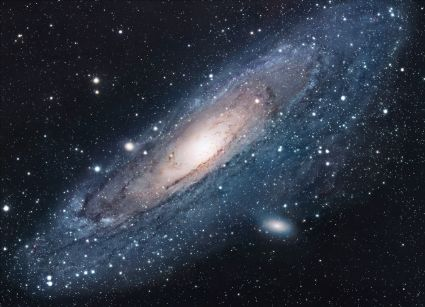
\includegraphics[scale=1.7]{universe}
% \caption{The Universe}
% \label{fig:universe}
% \end{figure}

% \section{Conclusion}
% ``I always thought something was fundamentally wrong with the universe'' \citep{adams1995hitchhiker}
% 
% \bibliographystyle{plain}
% \bibliography{references}

\section{First Part}
is here
\subsection{Instantaneous Velocity}

\subsection{Defining Instantaneous Velocity Using the Idea of a Limit}
\vfill
\section{Introduction}
\subsection{Purpose}
\paragraph{}
This document focuses on Requirements Analysis and Specification Document (RASD) and contains the description of the main goals, the domain and its representation through some models, the analysis of the scenario with the uses cases that describe them, the list of the most important requirements and specifications that characterize the development of the software described below.

\paragraph{}
It also includes the research about the interfaces, functional and non-functional requirements and the attributes that distinguish the quality of the system.

\paragraph{}
This document has the purpose to guide the developer in the realization of the software called CLup, a Customers Line-up application.

\paragraph{}
Finally, to understand better the development of the document, it contains the history that describes how it is made, with the references used and the description of its structure.

% table 
\begin{table}[hbt!]
\begin{tabular}{ l | l}
\hline
    \textbf{G1} & 2 \\  \hline
    \rowcolor[HTML]{34CDF9} salam & hi \\
    khobi & merCmerCmerCmerCmerCmerCmerCmerC \\ \hline
\end{tabular}
\end{table}

\subsection{Scope}
\subsection{Definition, Acronyms, Abbreviations}
\subsection{Revision history}
\subsection{Reference Documents}
\subsection{Document Structure}
\vfill
\end{document}
